\begin{frame}{General}

\begin{itemize}
\itemsep1pt\parskip0pt\parsep0pt
\item
  A two-weeks course, 1--12 June 2015.
\item
  18 participants from nine countries
\end{itemize}

\includegraphics{sem_files/figure-beamer/part-1.pdf}

\begin{itemize}
\itemsep1pt\parskip0pt\parsep0pt
\item
  Teachers: GB, EL, MJ, JJ.
\item
  Guest lecturers: SE, GS, JV, WL
\end{itemize}

\end{frame}

\begin{frame}{The participants and teachers}

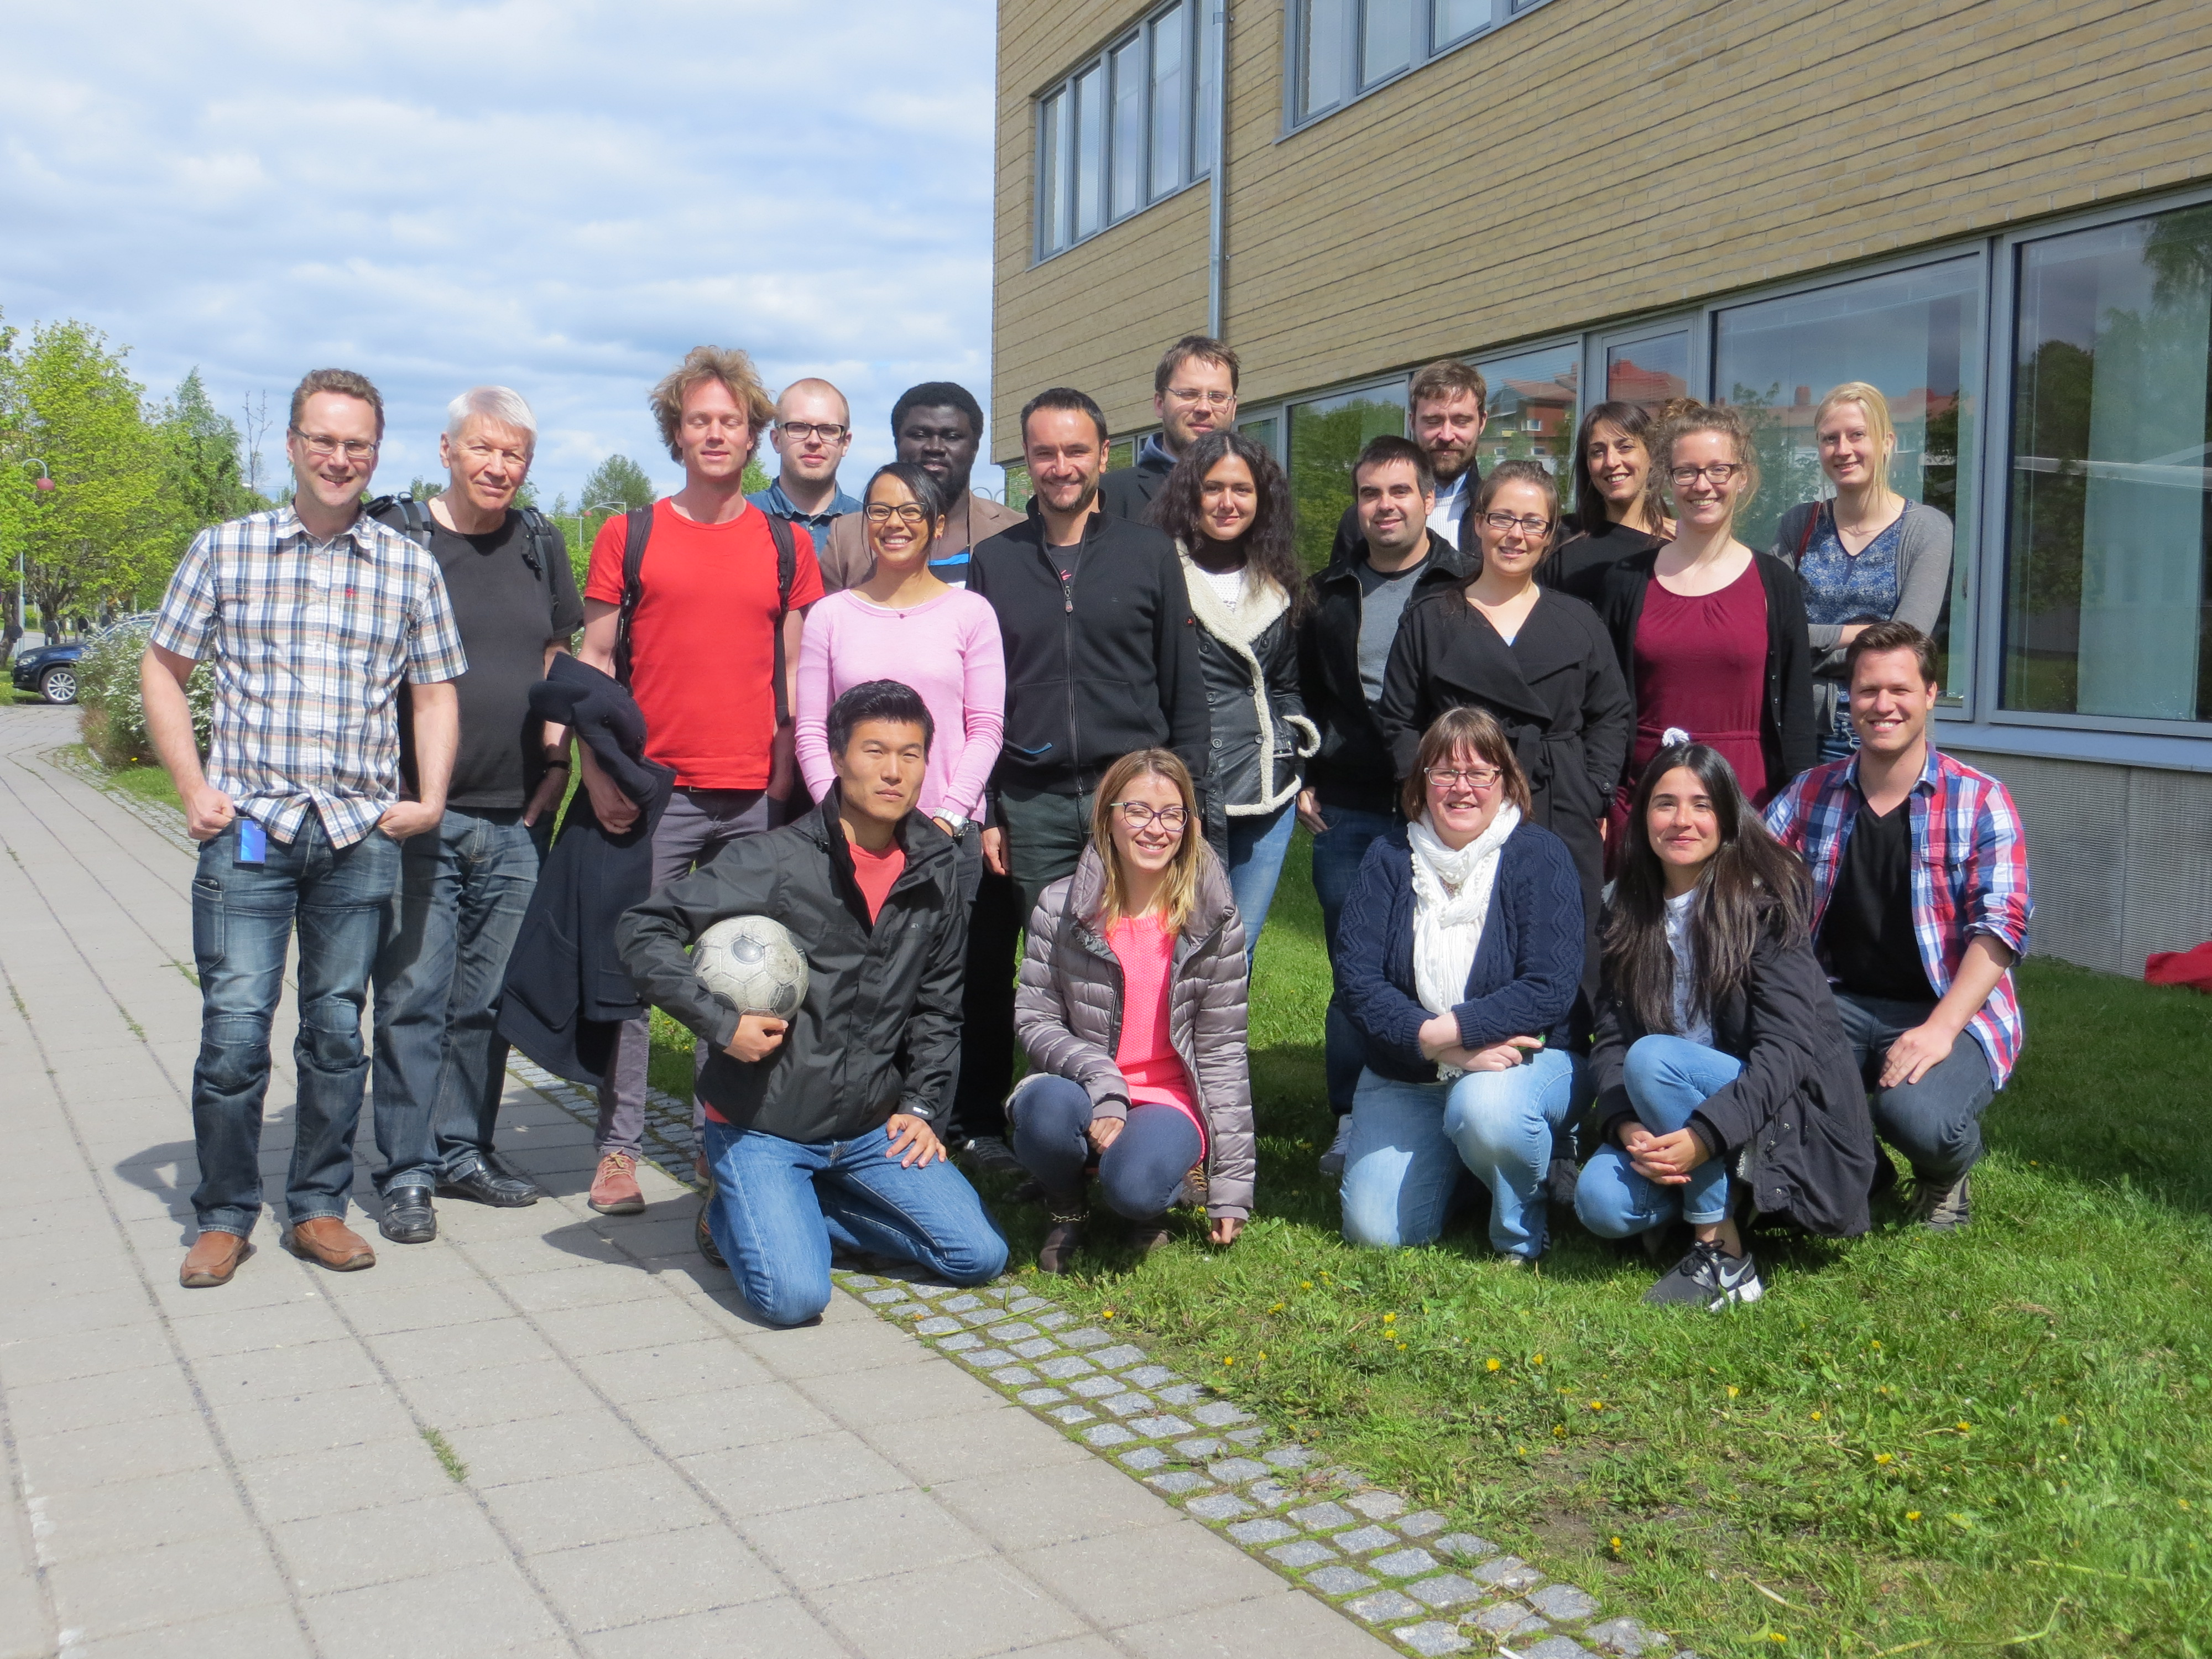
\includegraphics{figures/IMG_1780.JPG}

\end{frame}

\begin{frame}{General (cont'd)}

\begin{itemize}
\itemsep1pt\parskip0pt\parsep0pt
\item
  Organized by

  \begin{itemize}
  \itemsep1pt\parskip0pt\parsep0pt
  \item
    The European Historical Population Samples Network (EHPS-Net),
  \item
    The Graduate School in Population Dynamics and Public Policy
    (GSPDPP), and
  \item
    the Centre for Demographic and Ageing Research (CEDAR)
  \end{itemize}
\item
  under the auspices of European Science Foundation (ESF).
\item
  No tuition fee and some costs for participants were covered:

  \begin{itemize}
  \itemsep1pt\parskip0pt\parsep0pt
  \item
    The GSPDPP covered lodging costs for all participants,
  \item
    The ESF provided scholarships (for travel). Given to five
    participants.
  \end{itemize}
\end{itemize}

\end{frame}

\begin{frame}{Why R?}

\begin{enumerate}
\def\labelenumi{\arabic{enumi}.}
\itemsep1pt\parskip0pt\parsep0pt
\item
  R is \emph{free}.

  \begin{itemize}
  \itemsep1pt\parskip0pt\parsep0pt
  \item
    as in free beer
  \item
    as in free research
  \end{itemize}
\item
  R is open-source
\item
  R has over 6000 add-on packages
\item
  R will be the world leading statistical software.
\end{enumerate}

\end{frame}

\begin{frame}{Number of R packages on CRAN}

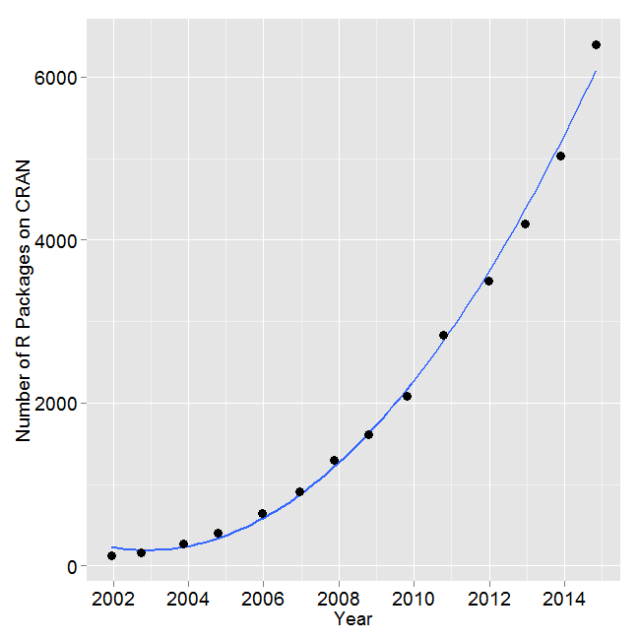
\includegraphics{figures/fig_9_cran.png}

Source: \url{http://r4stats.com}

\end{frame}

\begin{frame}{Why RStudio?}

Literate programming (Knuth, 1984):

\begin{itemize}
\item
  Dynamic report (paper) writing, programming, and documentation in one.
\item
  Automates \emph{reproducible research}.
\item
  Easy to combine with \emph{version control}.

  \begin{itemize}
  \itemsep1pt\parskip0pt\parsep0pt
  \item
    GitHub:\\\href{http://github.com/goranbrostrom/cedar/}{cedar}
  \end{itemize}
\end{itemize}

\end{frame}

\begin{frame}{More information}

Navigate to course home page

\href{http://capa.ddb.umu.se/cedar15}{\url{http://capa.ddb.umu.se/cedar15}}

\end{frame}

\begin{frame}{Statistical issues}

\begin{enumerate}
\def\labelenumi{\arabic{enumi}.}
\itemsep1pt\parskip0pt\parsep0pt
\item
  Interactions

  \begin{itemize}
  \itemsep1pt\parskip0pt\parsep0pt
  \item
    centering
  \item
    Presentation of results
  \end{itemize}
\item
  Omitted covariates in PH regression

  \begin{itemize}
  \itemsep1pt\parskip0pt\parsep0pt
  \item
    Don't!
  \end{itemize}
\item
  Causality and matching
\item
  The Hauck-Donner effect

  \begin{itemize}
  \itemsep1pt\parskip0pt\parsep0pt
  \item
    Bann the Wald \(p\)-values and significance stars!
  \end{itemize}
\end{enumerate}

\end{frame}

\begin{frame}{Interaction}

Data from Skellefteå: Old age mortality,

\begin{itemize}
\item
  ses and
\item
  birthdate
\item
  with interaction

  \begin{longtable}[c]{@{}lllll@{}}
  \toprule
  & coef exp & (coef) se( & coef) Pr( &
  \textgreater{}\textbar{}z\textbar{})\tabularnewline
  \midrule
  \endhead
  sesupper & -53.514 & 0.000 & 39.767 & 0.178\tabularnewline
  birthdate & 0.016 & 1.016 & 0.014 & 0.252\tabularnewline
  sesupper:birthdate & 0.029 & 1.030 & 0.022 & 0.182\tabularnewline
  \bottomrule
  \end{longtable}
\end{itemize}

\end{frame}

\begin{frame}[fragile]{Center birthdate around 1810}

\begin{Shaded}
\begin{Highlighting}[]
\NormalTok{mort$birthdate <-}\StringTok{ }\NormalTok{mort$birthdate -}\StringTok{ }\DecValTok{1810}
\end{Highlighting}
\end{Shaded}

\begin{longtable}[c]{@{}lrrrr@{}}
\toprule
& coef & exp(coef) & se(coef) &
Pr(\textgreater{}\textbar{}z\textbar{})\tabularnewline
\midrule
\endhead
sesupper & -0.558 & 0.572 & 0.134 & 0.000\tabularnewline
birthdate & 0.016 & 1.016 & 0.014 & 0.252\tabularnewline
sesupper:birthdate & 0.029 & 1.030 & 0.022 & 0.182\tabularnewline
\bottomrule
\end{longtable}

\begin{longtable}[c]{@{}lrrrr@{}}
\toprule
& Df & AIC & LRT & Pr(\textgreater{}Chi)\tabularnewline
\midrule
\endhead
& NA & 3687.529 & NA & NA\tabularnewline
ses:birthdate & 1 & 3687.319 & 1.7899 & 0.1809\tabularnewline
\bottomrule
\end{longtable}

\end{frame}

\begin{frame}{No interaction}

\begin{longtable}[c]{@{}lrrrr@{}}
\toprule
& coef & exp(coef) & se(coef) &
Pr(\textgreater{}\textbar{}z\textbar{})\tabularnewline
\midrule
\endhead
sesupper & -0.484 & 0.616 & 0.121 & 0.000\tabularnewline
birthdate & 0.029 & 1.029 & 0.011 & 0.008\tabularnewline
\bottomrule
\end{longtable}

\begin{longtable}[c]{@{}lrrrr@{}}
\toprule
& Df & AIC & LRT & Pr(\textgreater{}Chi)\tabularnewline
\midrule
\endhead
& NA & 3687.319 & NA & NA\tabularnewline
ses & 1 & 3701.428 & 16.1095 & 1e-04\tabularnewline
birthdate & 1 & 3692.594 & 7.2752 & 7e-03\tabularnewline
\bottomrule
\end{longtable}

\end{frame}

\begin{frame}{Effect of upper vs.~lower SES, no centering (log scale)}

\includegraphics{sem_files/figure-beamer/pres1log4-1.pdf}

\end{frame}

\begin{frame}{Effect of upper vs.~lower SES, no centering}

\includegraphics{sem_files/figure-beamer/pres1next-1.pdf}

\end{frame}

\begin{frame}{Effect of upper vs.~lower SES, with centering (log scale)}

\includegraphics{sem_files/figure-beamer/pres1log2-1.pdf}

\end{frame}

\begin{frame}{Effect of upper vs.~lower SES, with centering}

\includegraphics{sem_files/figure-beamer/pres12-1.pdf}

\end{frame}

\begin{frame}{Omitted covariates, example (simulated data)}

\begin{longtable}[c]{@{}rlll@{}}
\toprule
time & death & gender & civ\tabularnewline
\midrule
\endhead
13.010204 & TRUE & woman & married\tabularnewline
4.128730 & TRUE & woman & married\tabularnewline
45.268274 & TRUE & woman & married\tabularnewline
2.098910 & TRUE & woman & married\tabularnewline
8.002637 & TRUE & woman & married\tabularnewline
4.825463 & TRUE & woman & married\tabularnewline
\bottomrule
\end{longtable}

\end{frame}

\begin{frame}{Summary data}

Counts:

\begin{longtable}[c]{@{}lrr@{}}
\toprule
& married & unmarried\tabularnewline
\midrule
\endhead
woman & 1000 & 2000\tabularnewline
man & 2000 & 1000\tabularnewline
\bottomrule
\end{longtable}

Mean remaining life times (after 60):

\begin{longtable}[c]{@{}lrr@{}}
\toprule
& married & unmarried\tabularnewline
\midrule
\endhead
woman & 19.70 & 7.49\tabularnewline
man & 7.42 & 2.78\tabularnewline
\bottomrule
\end{longtable}

\end{frame}

\begin{frame}{Analysis (but wrong presentation!)}

\begin{table}[!htbp] \centering 
  \caption{} 
  \label{} 
\scriptsize 
\begin{tabular}{@{\extracolsep{5pt}}lcc} 
\\[-1.8ex]\hline 
\hline \\[-1.8ex] 
 & \multicolumn{2}{c}{\textit{Dependent variable:}} \\ 
\cline{2-3} 
\\[-1.8ex] & \multicolumn{2}{c}{time} \\ 
\\[-1.8ex] & (1) & (2)\\ 
\hline \\[-1.8ex] 
 genderman & 0.582$^{***}$ & 0.980$^{***}$ \\ 
  & (0.027) & (0.030) \\ 
  & & \\ 
 civunmarried &  & 0.970$^{***}$ \\ 
  &  & (0.030) \\ 
  & & \\ 
\hline \\[-1.8ex] 
Observations & 6,000 & 6,000 \\ 
Log Likelihood & $-$45,967.160 & $-$45,436.630 \\ 
\hline 
\hline \\[-1.8ex] 
\textit{Note:}  & \multicolumn{2}{r}{$^{*}$p$<$0.1; $^{**}$p$<$0.05; $^{***}$p$<$0.01} \\ 
\end{tabular} 
\end{table}

\end{frame}

\begin{frame}{Simpson's paradox!}

(Exponential distribution)

\[
\text{Relative Bias} \approx \frac{(n_{11} \alpha + n_{12})(n_{21} + n_{22})}{(n_{11} + n_{12})(n_{21} \alpha + n_{22})}
\] \includegraphics{sem_files/figure-beamer/relbi-1.pdf}

\end{frame}

\begin{frame}{Infant and maternal mortality}

Matched, left-truncated data (four first rows). 35 infants whose mothers
died. Two controls for each.

\begin{longtable}[c]{@{}rrrrl@{}}
\toprule
stratum & enter & exit & event & mother\tabularnewline
\midrule
\endhead
1 & 55 & 365 & 0 & dead\tabularnewline
1 & 55 & 365 & 0 & alive\tabularnewline
1 & 55 & 365 & 0 & alive\tabularnewline
2 & 13 & 76 & 1 & dead\tabularnewline
\bottomrule
\end{longtable}

\begin{longtable}[c]{@{}rllllr@{}}
\toprule
age & sex & parish & civst & ses & year\tabularnewline
\midrule
\endhead
26 & boy & Nedertornea & married & farmer & 1877\tabularnewline
26 & boy & Nedertornea & married & farmer & 1870\tabularnewline
26 & boy & Nedertornea & married & farmer & 1882\tabularnewline
23 & girl & Nedertornea & married & other & 1847\tabularnewline
\bottomrule
\end{longtable}

\end{frame}

\begin{frame}[fragile]{The analysis}

Stratify!

\begin{Shaded}
\begin{Highlighting}[]
\NormalTok{fit <-}\StringTok{ }\KeywordTok{coxreg}\NormalTok{(}\KeywordTok{Surv}\NormalTok{(enter, exit, event) ~}\StringTok{ }\NormalTok{mother +}\StringTok{ }
\StringTok{                  }\KeywordTok{strata}\NormalTok{(stratum), }\DataTypeTok{data =} \NormalTok{infants)}
\NormalTok{dr <-}\StringTok{ }\KeywordTok{drop1}\NormalTok{(fit, }\DataTypeTok{test =} \StringTok{"Chisq"}\NormalTok{)}
\KeywordTok{ltx}\NormalTok{(fit, }\DataTypeTok{dr =} \NormalTok{dr, }\DataTypeTok{digits=}\DecValTok{4}\NormalTok{)}
\end{Highlighting}
\end{Shaded}

\begin{table}[ht] 
\begin{center} 
\begin{tabular}{lrrrrr} 
\hline 
Covariate & Mean & Coef & Rel.Risk & S.E. &   L-R p \\ \hline
mother  & & & & & 0.0000  \\ 
\multicolumn{1}{r}{\em alive} &   0.7628 & 0 & 1 & \multicolumn{2}{c}{(reference)} \\ 
\multicolumn{1}{r}{ \em dead }  &    0.2372  &  2.6052  &  13.5344  &  0.7567\\ 
\hline 
Events &  21  & TTR &  21616 \\ 
Max. Log Likelihood &  -10.81 \\ \hline 
\hline 
\end{tabular}
\end{center} 
\end{table}

\end{frame}

\begin{frame}{References}

Broström, G. (1987), The influence of mother's mortality on infant
mortality. \emph{Scandinavian Journal of Statistics} \textbf{14},
251--261.

Broström, G. (2012). \emph{Event History Analysis with R.} CRC
Press/Chapman \& Hall, Boca Raton, CA, USA.

\end{frame}

\begin{frame}{The two-sample problem (example)}

\includegraphics{sem_files/figure-beamer/whyma-1.pdf}

Statistically significant difference?

\end{frame}

\begin{frame}[fragile]{The t-test}

\scriptsize

\begin{Shaded}
\begin{Highlighting}[]
\KeywordTok{t.test}\NormalTok{(X, Y)}
\end{Highlighting}
\end{Shaded}

\begin{verbatim}
## 
##  Welch Two Sample t-test
## 
## data:  X and Y
## t = -1.6337, df = 18, p-value = 0.1197
## alternative hypothesis: true difference in means is not equal to 0
## 95 percent confidence interval:
##  -13.568821   1.697458
## sample estimates:
## mean of x mean of y 
##  7.645328 13.581009
\end{verbatim}

\end{frame}

\begin{frame}{Paired data}

\includegraphics{sem_files/figure-beamer/pairda-1.pdf}

\end{frame}

\begin{frame}[fragile]{The paired t-test}

\scriptsize

\begin{Shaded}
\begin{Highlighting}[]
\KeywordTok{t.test}\NormalTok{(X, Y, }\DataTypeTok{paired =} \OtherTok{TRUE}\NormalTok{)}
\end{Highlighting}
\end{Shaded}

\begin{verbatim}
## 
##  Paired t-test
## 
## data:  X and Y
## t = -109.19, df = 9, p-value = 2.3e-15
## alternative hypothesis: true difference in means is not equal to 0
## 95 percent confidence interval:
##  -6.058649 -5.812713
## sample estimates:
## mean of the differences 
##               -5.935681
\end{verbatim}

\normalsize

The sign test: p = 2 * .5\^{}10 = 0.00195 (two-sided)

\end{frame}

\begin{frame}{The `Hauck-Donner effect' (example)}

\includegraphics{sem_files/figure-beamer/hdata-1.pdf}

\end{frame}

\begin{frame}[fragile]{Linear regression, code}

\begin{Shaded}
\begin{Highlighting}[]
\KeywordTok{options}\NormalTok{(}\DataTypeTok{show.signif.stars =} \OtherTok{FALSE}\NormalTok{)}
\NormalTok{fit <-}\StringTok{ }\KeywordTok{lm}\NormalTok{(T ~}\StringTok{ }\NormalTok{x, }\DataTypeTok{data =} \NormalTok{dat)}
\KeywordTok{summary}\NormalTok{(fit)}
\end{Highlighting}
\end{Shaded}

\end{frame}

\begin{frame}[fragile]{Linear regression, results}

\scriptsize

\begin{verbatim}
## 
## Call:
## lm(formula = T ~ x, data = dat)
## 
## Residuals:
##      Min       1Q   Median       3Q      Max 
## -0.12247 -0.11609 -0.09949 -0.08289  0.91786 
## 
## Coefficients:
##             Estimate Std. Error t value Pr(>|t|)
## (Intercept)  0.12758    0.23077   0.553    0.595
## x            0.99489    0.03773  26.365  4.6e-09
## 
## Residual standard error: 0.3425 on 8 degrees of freedom
## Multiple R-squared:  0.9886, Adjusted R-squared:  0.9872 
## F-statistic: 695.1 on 1 and 8 DF,  p-value: 4.603e-09
\end{verbatim}

\end{frame}

\begin{frame}[fragile]{ANOVA}

\begin{Shaded}
\begin{Highlighting}[]
\KeywordTok{anova}\NormalTok{(fit)}
\end{Highlighting}
\end{Shaded}

\begin{verbatim}
## Analysis of Variance Table
## 
## Response: T
##           Df Sum Sq Mean Sq F value    Pr(>F)
## x          1 81.561  81.561  695.14 4.603e-09
## Residuals  8  0.939   0.117
\end{verbatim}

\emph{Note} that the \textbf{F test} is appropriate for \emph{linear
models} (with unknown variance)

\end{frame}

\begin{frame}{Cox regression,}

Wald test:

\begin{table}[ht] 
\begin{center} 
\begin{tabular}{lrrrrr} 
\hline 
Covariate & Mean & Coef & Rel.Risk & S.E. &   Wald p \\ \hline
x  &     6.891  &  -5.884  &  0.003  &  6.628  & 0.375 \\ 
\hline 
Events &  10  & TTR &  55 \\ 
Max. Log Likelihood &  -0.84 \\ \hline 
\hline 
\end{tabular}
\end{center} 
\end{table}

LR test:

\scriptsize

\begin{table}[ht] 
\begin{center} 
\begin{tabular}{lrrrrr} 
\hline 
Covariate & Mean & Coef & Rel.Risk & S.E. &   L-R p \\ \hline
x  &  6.890545  &  -5.883515  &  0.002785  &  6.627865  & 0.000000 \\ 
\hline 
Events &  10  & TTR &  55 \\ 
Max. Log Likelihood &  -0.840062 \\ \hline 
\hline 
\end{tabular}
\end{center} 
\end{table}

\end{frame}

\begin{frame}{Cox regression, Likelihood Ratio Test}

\emph{Note} the \textbf{Hauck-Donner} (1977; \emph{JASA} \textbf{72}
851--853) effect!

Strikes in \emph{non-linear} models (not only Cox)!

\end{frame}

\begin{frame}{The ``graphical''" explanation}

\includegraphics{sem_files/figure-beamer/grapex-1.pdf}

\end{frame}

\begin{frame}{Wald and presentation (bad)}

\begin{table}[ht] 
\begin{center} 
\begin{tabular}{lrrrrr} 
\hline 
Covariate & Mean & Coef & Rel.Risk & S.E. &   Wald p \\ \hline
civ  \\ 
\multicolumn{1}{r}{\em unmarried} &    0.080 & 0 & 1 & \multicolumn{2}{c}{(reference)} \\ 
\multicolumn{1}{r}{ \em married }  &     0.530  &  -0.345  &  0.708  &  0.081 & 0.000\\ 
\multicolumn{1}{r}{ \em widow }  &     0.390  &  -0.259  &  0.772  &  0.080 & 0.001\\ 
region  \\ 
\multicolumn{1}{r}{\em town} &    0.111 & 0 & 1 & \multicolumn{2}{c}{(reference)} \\ 
\multicolumn{1}{r}{ \em industry }  &     0.326  &  0.298  &  1.347  &  0.086 & 0.001\\ 
\multicolumn{1}{r}{ \em rural }  &     0.563  &  0.152  &  1.164  &  0.084 & 0.070\\ 
\hline 
Events &  1971  & TTR &  37824 \\ 
Max. Log Likelihood &  -13563 \\ \hline 
\hline 
\end{tabular}
\end{center} 
\end{table}

\end{frame}

\begin{frame}{LR and presentation (good)}

\begin{table}[ht] 
\begin{center} 
\begin{tabular}{lrrrrr} 
\hline 
Covariate & Mean & Coef & Rel.Risk & S.E. &   L-R p \\ \hline
civ  & & & & & 0.0002  \\ 
\multicolumn{1}{r}{\em unmarried} &   0.0800 & 0 & 1 & \multicolumn{2}{c}{(reference)} \\ 
\multicolumn{1}{r}{ \em married }  &    0.5300  &  -0.3449  &  0.7083  &  0.0814\\ 
\multicolumn{1}{r}{ \em widow }  &    0.3900  &  -0.2592  &  0.7716  &  0.0797\\ 
region  & & & & & 0.0003  \\ 
\multicolumn{1}{r}{\em town} &   0.1111 & 0 & 1 & \multicolumn{2}{c}{(reference)} \\ 
\multicolumn{1}{r}{ \em industry }  &    0.3262  &  0.2977  &  1.3468  &  0.0856\\ 
\multicolumn{1}{r}{ \em rural }  &    0.5628  &  0.1521  &  1.1642  &  0.0839\\ 
\hline 
Events &  1971  & TTR &  37824 \\ 
Max. Log Likelihood &  -13563 \\ \hline 
\hline 
\end{tabular}
\end{center} 
\end{table}

\end{frame}

\begin{frame}{What could we do better?}

\begin{enumerate}
\def\labelenumi{\arabic{enumi}.}
\item
  Better synchronisation between teachers of R/RStudio!
\item
  More R/RStudio stuff the first week.

  \begin{itemize}
  \itemsep1pt\parskip0pt\parsep0pt
  \item
    More Johan J.!
  \end{itemize}
\item
  More exercises --- less project work.
\item
  One or two more lab assistants

  \begin{itemize}
  \itemsep1pt\parskip0pt\parsep0pt
  \item
    Negotiation with the statistics department broke down(?)
  \end{itemize}
\item
  Course evaluations were constructive and in general positive.

  \begin{itemize}
  \itemsep1pt\parskip0pt\parsep0pt
  \item
    Service and organisation of practical matters were \emph{excellent}!
    Thanks Annika!
  \end{itemize}
\end{enumerate}

\end{frame}
